\documentclass[tikz,border=8pt]{standalone}
\usepackage{fontspec}
\setsansfont{Arial}
\usetikzlibrary{arrows.meta,positioning}
\begin{document}
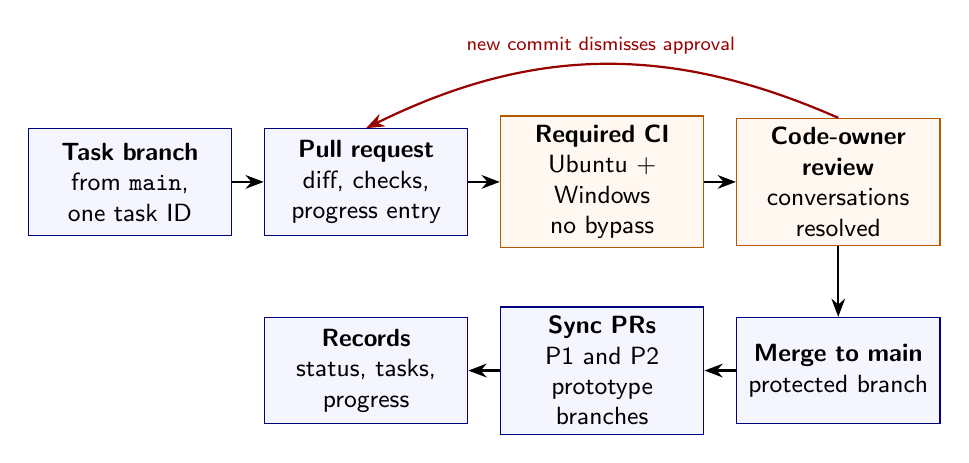
\begin{tikzpicture}[font=\sffamily\small,>=Stealth,
box/.style={draw=blue!50!black,align=center,text width=2.35cm,minimum height=1.35cm,fill=blue!4},
gate/.style={draw=orange!70!black,align=center,text width=2.35cm,minimum height=1.35cm,fill=orange!6}]
% Repository contribution workflow (Section 1.4.4), as configured under task T36.
\node[box] (b) {\textbf{Task branch}\\from \texttt{main},\\one task ID};
\node[box,right=0.4cm of b] (p) {\textbf{Pull request}\\diff, checks,\\progress entry};
\node[gate,right=0.4cm of p] (ci) {\textbf{Required CI}\\Ubuntu + Windows\\no bypass};
\node[gate,right=0.4cm of ci] (r) {\textbf{Code-owner review}\\conversations\\resolved};
\node[box,below=0.9cm of r] (m) {\textbf{Merge to main}\\protected branch};
\node[box,left=0.4cm of m] (s) {\textbf{Sync PRs}\\P1 and P2\\prototype branches};
\node[box,left=0.4cm of s] (d) {\textbf{Records}\\status, tasks,\\progress};
\draw[->,thick] (b)--(p);\draw[->,thick] (p)--(ci);\draw[->,thick] (ci)--(r);
\draw[->,thick] (r)--(m);\draw[->,thick] (m)--(s);\draw[->,thick] (s)--(d);
\draw[->,thick,red!60!black] (r.north) to[bend right=25] node[above,font=\sffamily\scriptsize]{new commit dismisses approval} (p.north);
\end{tikzpicture}
\end{document}
